\section{A Project Inspiration: JTAG to DE10-Lite Interface}

The inspiration for this project came from a a search at github.com on DE10-Lite:

\url{https://github.com/hildebrandmw/de10lite-hdl}

This is a nice collection of work done with the DE10-Lite board for academic purposes.
What really got my attention is the project play\_gif:

\url{https://github.com/hildebrandmw/de10lite-hdl/tree/master/projects/play_gif}

The interesting feature of this project is the usage of the USB to load data (animated GIF image file)
to the FPGA.  So this is a data pipeline from a Linux desktop to the FPGA which is built into the board!
This met my requirement that I be able to control the FPGA remotely from a desktop (or SBC) computer.

The interface is via ``JTAG'', which is typically used as a debugging interface.  It is not specifically intended for mass data transfer, but in this case it was pressed into service.

The interface is a bit clunky to use.  It requires a ``TCL Server'', and a running instance of the Quartus development tool!  Not exactly what I was looking for, but I got the demo to work easily!  It is very nicely done work demonstrating several features of FPGA technology.

The way it works is conceptually simple.  The FPGA part of the project implements a VGA\footnote{VGA is a relatively simple video standard which seems to be common on many FPGA development boards.} interface to the connector on the DE10-Lite board.  The image loaded from the desktop computer is sliced into its constituent ``frames''.
Another interesting aspect of the project is the interface to the SDRAM of the DE10-Lite which is a 64MB external part on the board.  The sliced-up image is loaded into the SDRAM, and then another control module pages the VGA output through the memory.  Thus you see the animated GIF displayed on the monitor.  Really you are seeing in a very direct manner the data loaded into the SDRAM.  Cool!

\subsection{IP and Platform Designer}

First, a little bit of FPGA jargon.  ``Intellectual Property'' (IP) in the context of semiconductor devices is a block of circuitry which has been heavily engineered and refined to perform some particular function.  It could be patented or otherwise protected from duplication by competitors.
Due to the way integrated circuits are manufactured, blocks of ''IP'' can be added to the silicon and be expected to perform to the IP owner's specifications.  Typically IP can be included as part of a design kit, or it can be paid for with a license fee.

IP is good because it can reduce engineering design effort, improve performance, and enhance quality.  The trade-off is license fee cost, and you don't necessarily get exactly what you want.

In our case, we are given a whole bunch of IP for free that we can experiment with!  This is bundled into ``Platform Designer'' which is a tool-within-a-tool in the Quartus design suite.

To do justice to this there should be an entire section on ``Platform Designer''.  I will summarize here.  There are excellent video Platform Designer tutorials which you can access if you register for a free account at the Intel web site.

``Platform Designer'' is a building-block system.  You get a library of IP, along with a mechanism to hook them together.  The design is bundled into a ``Qsys'' file.    Let's have a look at the Qsys part of the play\_gif project:

\begin{figure}[h]
	\centering
	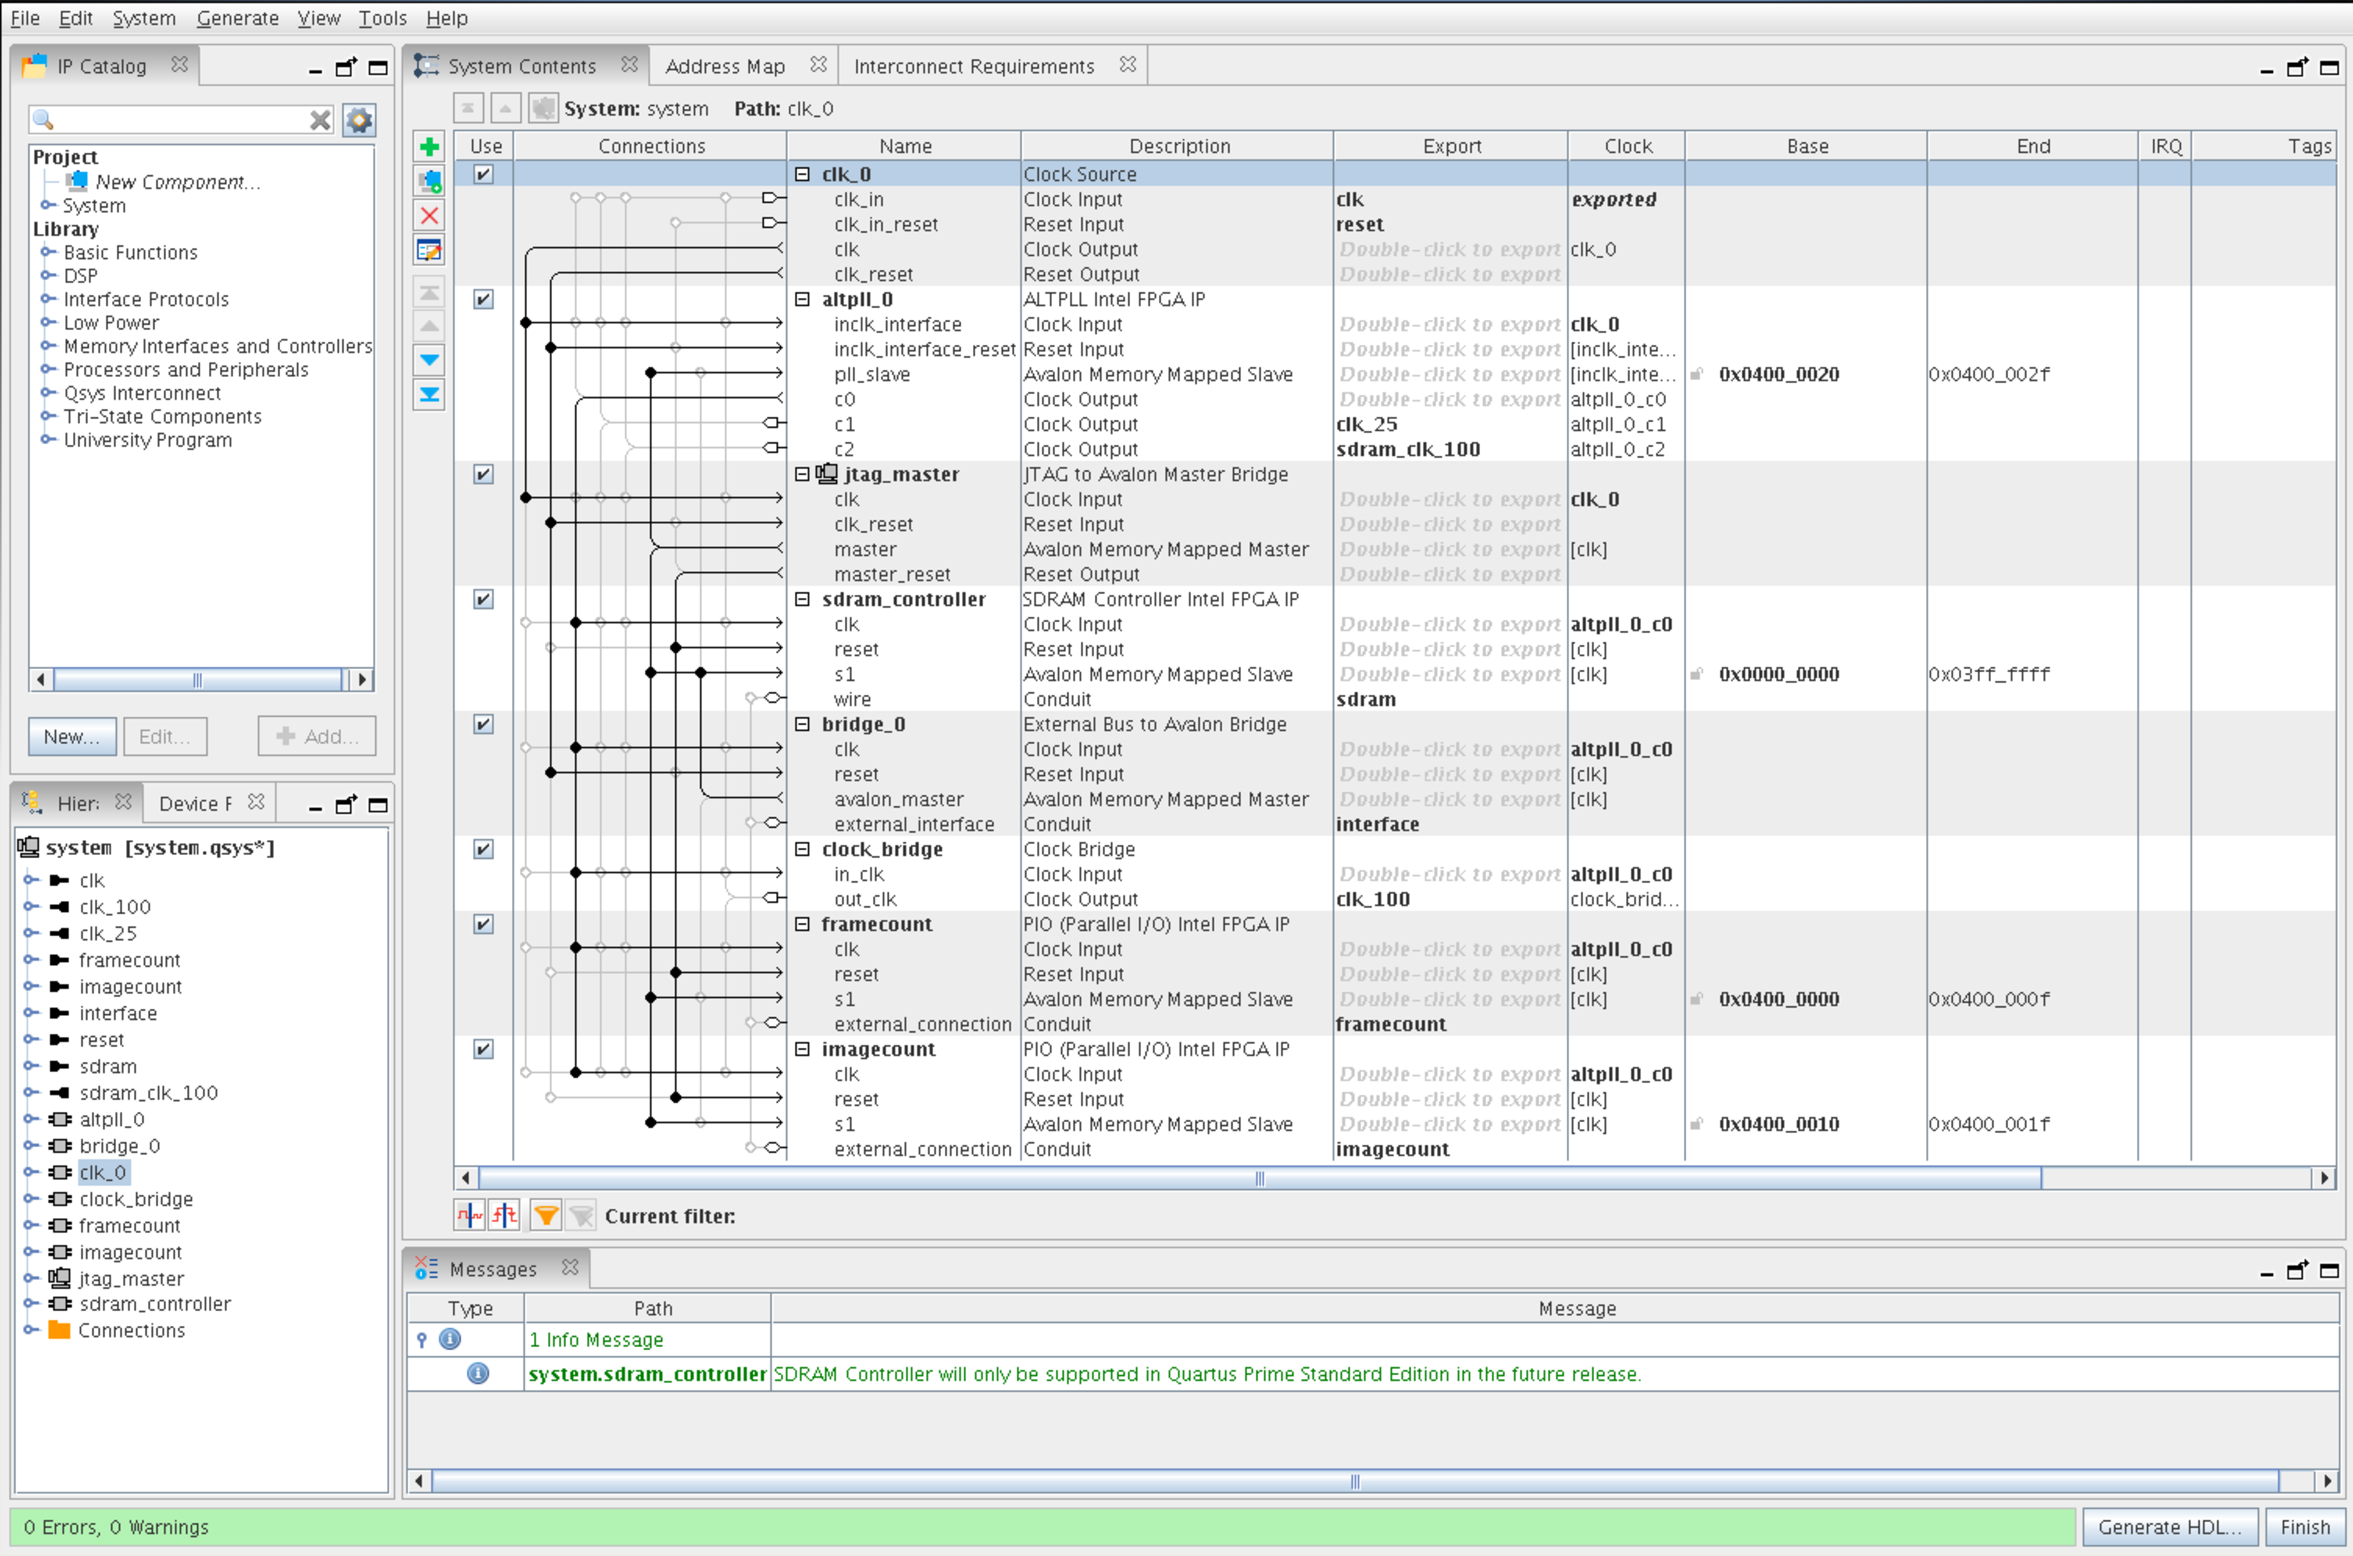
\includegraphics[width=1.0\textwidth]{images/platform_designer.pdf}
	\centering\bfseries
	\caption{Play\_gif project Qsys file}
\end{figure}

The upper left corner of the GUI is the library of IP.  Some of the categories:

\begin{itemize}
	\item Basic Functions
\item DSP
\item Memory Interfaces
\item Processors and Peripherals (including a ``Nios'' processor)
\item Memory Interfaces and Controllers
\end{itemize}

There is a sort of ``sub-library'' called  ``University Program'' which includes:

\begin{itemize}
	\item Audio and Video
\item Bridges
\item Clocks
\item Communication
\item Generic IO
\item Memory
\end{itemize}

The project used this IP:

\begin{enumerate}
\item ALTPLL Intel FPGA IP
\item JTAG to Avalon Master Bridge
\item DRAM Controller Intel FPGA IP
\item External Bus to Avalon Bridge
\item Clock Bridge
\item (Parallel IO) Intel FPGA IP
\end{enumerate}

The above IP can be seen in the column ``Name''.  There are two instantiations of the Parallel IO.
In the column ``Connections'' can be seen the graphical interconnections between the IP blocks.
Connections are made by simply clicking on the circles at the intersections of the ``wires'' between the IP.
Thus an entire system can be assembled using this GUI.  No writing of Verilog required!
The project does include some hand-written Verilog.  This ``Qsys'' design is ``dropped in'' to the project
as a Verilog module.

Here is what the system looks like:

\begin{figure}[h]
	\centering
	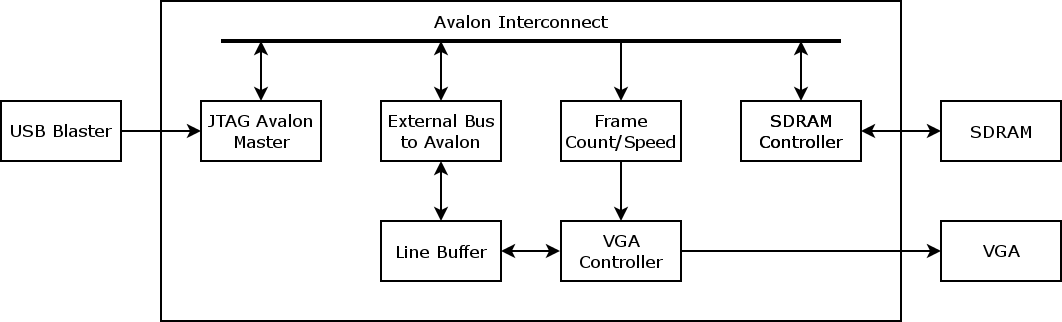
\includegraphics[width=1.0\textwidth]{images/play_gif.png}
	\centering\bfseries
	\caption{Play\_gif JTAG Interface System Diagram}
\end{figure}

What this diagram does not show is the requirement for a running Quartus and a TCL/JTAG server program.

The ``Avalon Interconnect'' deserves some explanation.  This is a system bus used in the MAX10 FPGA.  From the Avalon Interface specification:

\begin{quotation}
	Avalon® interfaces simplify system design by allowing you to easily connect
components in Intel® FPGA. The Avalon interface family defines interfaces appropriate
for streaming high-speed data, reading and writing registers and memory, and
controlling off-chip devices. Components available in Platform Designer incorporate
these standard interfaces. Additionally, you can incorporate Avalon interfaces in
custom components, enhancing the interoperability of designs.
\end{quotation}

It is an internal bus standard used to connect Avalon bus masters and slaves.  So it is a single-click process to connect Avalon components in Platform Designer.  It is really amazing what you get for such little effort!

This project is interesting, and shows a path to communication between a desktop computer and the FPGA.
However, the JTAG + Quartus + TCL/JTAG Server is cumbersome.  A SPI to Avalon bus IP component is listed in the catalog.
What if the JTAG and development tools could be replaced by something simpler like a SPI bus?

So that is what evolved into my ``introductory FPGA project''.  The revised system diagram:

\begin{figure}[h]
	\centering
	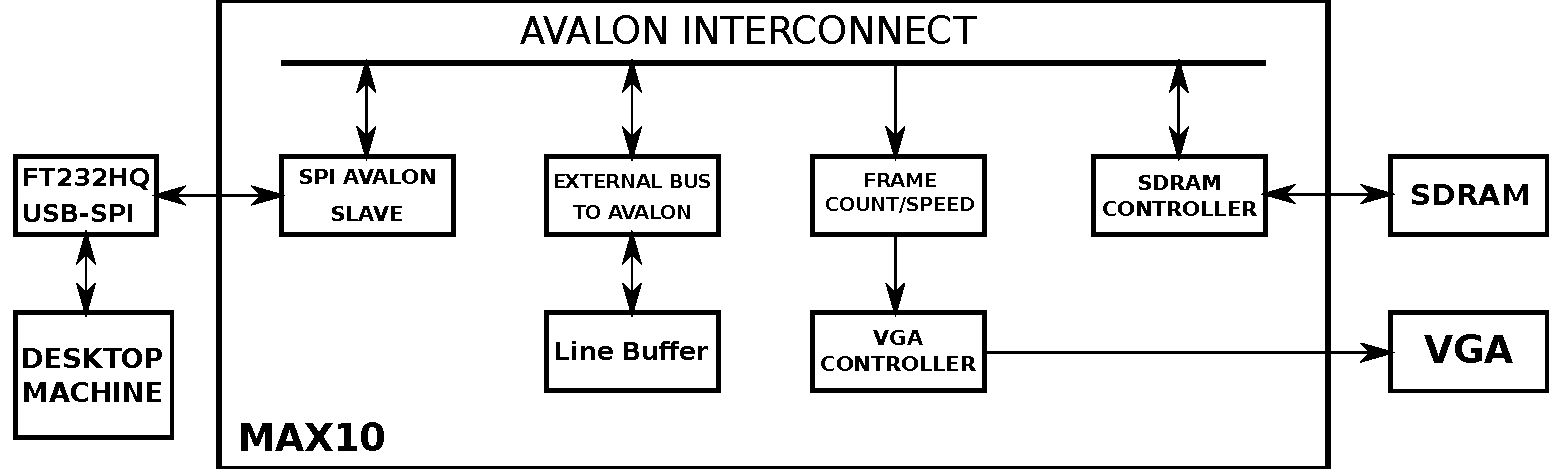
\includegraphics[width=1.0\textwidth]{images/spi_avalon_system}
	\centering\bfseries
	\caption{Play\_gif with SPI System Diagram}
\end{figure}

The significant change on the FPGA is the swapping of the JTAG Avalon bus master with the SPI-Avalon slave.  This was not entirely a drop-in replacement, as there were changes to reset and clock connections in addition to swapping JTAG to SPI components.  But it is easy, and the swapping can be done in a couple of minutes.

External to the DE10-Lite board, there is a USB to SPI adapter board.  This board is based on the FT232H chip by FTDI.  This can be bought from eBay for about \$10.  Search for ``ft232 spi'' and you will find several options.  I recommend one with headers to allow it to be plugged into a common breadboard.  The FTDI device requires a C shared library (libMPSSE) to be installed:

\url{https://www.ftdichip.com/Support/SoftwareExamples/MPSSE/LibMPSSE-SPI.htm}

Other changes required for SPI:

\begin{itemize}
	\item The ports on the QSYS module changed (JTAG -> SPI), thus the Verilog module in which it is instantiated required minor changes.  This was done with the text editor feature of Quartus.
    \item Another change is required to the FPGA pins.  The new SPI bus must be routed to some easily accessible header on the DE10-Lite board.  Since the board has an Arduino compatible header, and this header has a standard set of four pins for SPI, those pins were used.  The details can be seen in the DE10-Lite manual provided by Terasic.  The ``Pin Planner'' tool was used to make the changes.
    \item The ``Synopsys Design Constraints'' (.sdc) file was updated to incorporate the SPI bus.
\end{itemize}

Here is the rapid-prototype breadboard hook-up:

\begin{figure}[h]
	\centering
	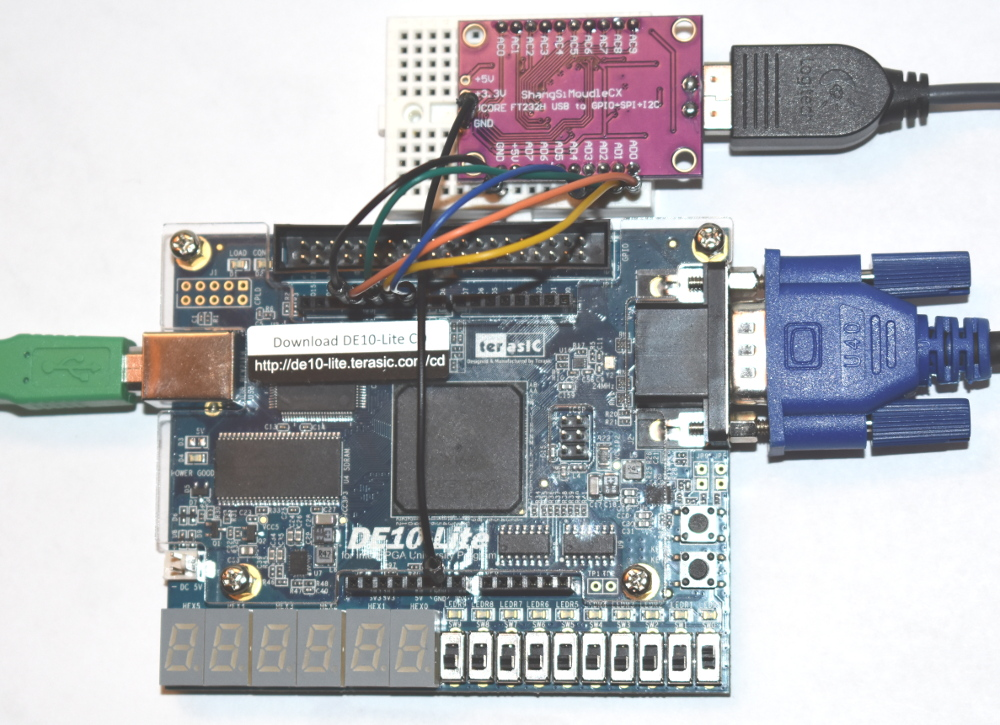
\includegraphics[width=0.5\textwidth]{images/de10_spi}
	\centering\bfseries
	\caption{DE10-Lite Connected to FTDI SPI Breakout}
\end{figure}

In spite of the length of the breadboard jumper wires, the SPI interface performed remarkably well right up to the FTDI clock limit of 30 MHz.









